\documentclass[11pt, a4paper]{article}
\usepackage[utf8x]{inputenc}
\usepackage[sort]{natbib}

\usepackage[spanish]{babel}
\usepackage{enumitem}
\usepackage{graphicx}
\usepackage{float}
\usepackage[linktoc=all]{hyperref}

\usepackage{etoolbox}

\usepackage{amsmath}
\usepackage{amssymb}
\usepackage{array}
\usepackage{gensymb}

\usepackage{fancyhdr}
\usepackage[table]{xcolor}
\usepackage{color}
\usepackage{colortbl}
\definecolor{lightgray}{gray}{0.9}
\setlength{\columnsep}{0.5cm}


%------------------- Dimensiones -------------------
\usepackage{geometry}
 \geometry{a4paper,total={170mm,257mm},left=15mm,right=15mm,top=20mm,}
%----------------------------------------------------

%------------------- Encabezado y Pie de pág -------------------
\pagestyle{fancy}
\fancyhf{}
\lhead{Técnicas Digitales IV}
\rhead{TP3}
\rfoot{Página \thepage}
%----------------------------------------------------


%----------------------------- Documento -----------------------------------------------
\begin{document}
\begin{titlepage}
 \centering
	
\includegraphics[scale=0.80]{Imagenes/LOGO.jpg} \par
 	\vspace{1cm}
 	{\scshape\LARGE Universidad Tecnológica Nacional \par}
 	{\scshape\large Facultad Regional de Córdoba \par}
 	\vspace{1cm}
	{\bfseries \Large Trabajo Práctico De Laboratorio $N^{\circ} 3$\par}
 	\vspace{1.5cm}

	\begin{tabular}{ll}
		Navarro, Facundo		&	63809 	
	\end{tabular}
	
	\vspace{1cm}
	Curso: 6r4 \\
	Grupo $N^{\circ} 5$
 	\vfill
	{\bfseries \Large Técnicas Digitales IV\par}

	\vspace{1.5cm}
	Docentes: \par
	Ing. Cayuela, Pablo \par
	Ing. Olmedo, Sergio \par

 	\vfill
	{\large \today\par}
\end{titlepage}
	
	
\tableofcontents
\clearpage

\section{Introducción}
En el siguiente trabajo práctico se investigan e implementan protocolos de comunicación síncronos, en donde $R_X$ y $T_X$ operan en conjunto con un señal de $clock$, los cuales son $I^{2}C$, $SPI$, $PS2$.

\section{Desarrollo}
	\subsection{Personal system version 2 (PS2)}


	\subsection{Inter intergrated circuit ($I^{2}C$)}
		Es un bus serial de comunicación de 8 bits entre circuitos integrados que se encuentran próximos entre ellos (normalmente en la misma placa). Utiliza tan solo dos cables (mas GND de referencia) y tiene cuatro modos estandarizados de velocidad
		\begin{itemize} \itemsep0em
			\item standard (100 kbps)
			\item fast (400 kbps)
			\item fast-plus (1 Mbps)
			\item high-speed (3,3 Mbps)
		\end{itemize}

		El bus $I^{2}C$ consisten en dos cables, llamados \textit{SCL} (serial clock) y \textit{SDA} (serial data), los cuales interconectan un \textit{master} con un número de unidades \textit{esclavas}.Cada dispositivo en el bus tiene una única dirección y puede operar como transmisor o receptor, poniendo o adquiriendo datos en la linea \textit{SDA}, es decir que esta linea es bidireccional. El clock es unidireccional y es generado por el master, quien además es el encargado de iniciar y finalizar la transferencia de datos. Ejemplos de familias de integrados actualmente fabricados con soporte $I^{2}C$ son: memorias flash y EEPROM, conversores A/D y D/A, circuitos RTC, sensores de temperatura, etc.
		
		Las salidas de SCL y SDA son a  drenador abierto, por lo que son necesarias resistencias del tipo pull-up ($R_{UP}$), normalmente en el rango de los 1,5 a 33 $k\Omega$. El valor de $R_{UP}$ depende de la capacitancia total del nodo, en caso de buses muy largos con muchos esclavos adheridos a él, entonces las resistencias deben ser pequeñas para alcanzar el mínimo ``rise time" definido en la especificaciones del $I^{2}C$.

		El número de dispositivos compartiendo el mismo bus puede alcanzar hasta 128 (direcciones de 7-bit) o 1024 (direcciones de 10-bit). Más de un \textit{master} es permitido, el tal caso el protocolo $I^{2}C$ administra el bus, considerando como master principal al primero que ponga el bajo el voltaje de \textit{SDA}.

		\subsubsection{Operación de la interfaz $I^{2}C$}
			El diagrama de tiempos de una típica transferencia de datos se muestra en la figura \textcolor{blue}{\textbf{\ref{fig:basic_timing}}}. Ambas lineas estan en alto cuando el bus esta en estado ``inactivo". El master inicia la transferencia creando una condición de arranque (S), en la cual SDA cambia de alto a bajo mientras que SCL se mantiene en alto. Luego genera la señal clock sobre SCL. Dependiendo del tipo de transacción, o el maestro o el esclavo seleccionado introducen datos sobre SDA. Los datos deben ser estables cuando SCL este en alto y el cambio de dato solo puede ocurrir cuando SCL este en bajo. Estas definiciones aseguran que tanto las condiciones de arranque como parada nunca puedan ser confundidas como datos.
			
		\begin{figure}[H]
			\centering
			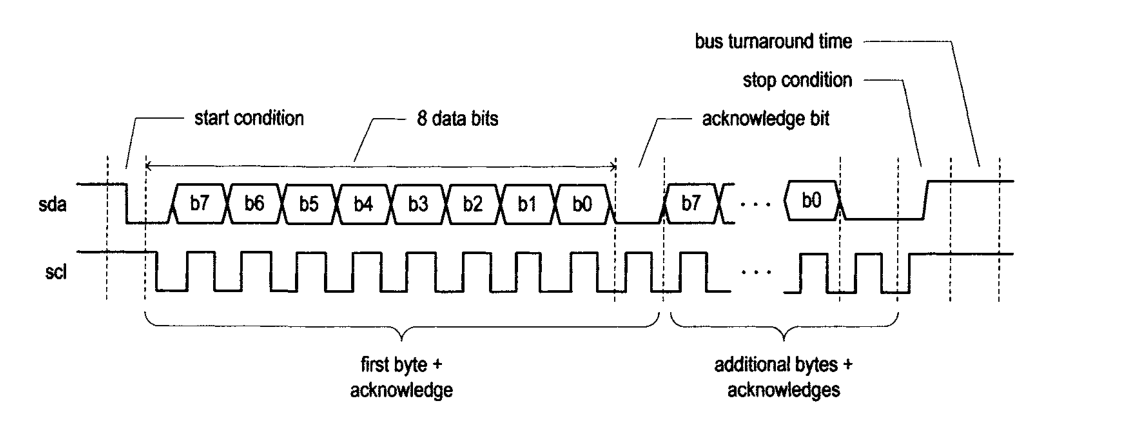
\includegraphics[width=0.6\textwidth]{Imagenes/basic_timing.png}
			\caption{Diagrama de tiempos genérico de una transferencia por $I^{2}C$}
			\label{fig:basic_timing}
		\end{figure} 

			La transferencia esta hecha byte-a-byte con el MSB primero. Cada byte es seguido con un ``acknowledge" bit en el noveno pulso de reloj. El número de bytes en una transferencia no está restringido. Después de terminado, el master finaliza la transferencia creando una condición de parada (P), en la cual SDA cambia de bajo a alto mientras SCL se mantiene en alto. Luego de que la transferencia esta completada el bus debe esperara un pequeño tiempo (turnaround time) antes de inicializar otra transacción.
	\subsection{Serial peripheral interface (SPI)}

\end{document}
